\section{Experiments}\label{sec:experiments}

\todo{Left to do: uniformise "mean orientation error" in the text with chosen notation.}

% \begin{itemize}
%     %\item \lau{Put pas tense everywhere.} done
%     %\item \todo{Update throughout (also in figures): $E \rightarrow E_\text{OR}, OR \rightarrow L_\text{OR}$, and use $L_\text{DE}$.} done
%     %\item \mdeff{In general, we should try to make the text in figures larger. A trick I use in matplotlib is to lower the figure size, e.g., \texttt{fig = %plt.figure(figsize=(4, 4))}}.done
%     %\item \mdeff{We now have one figure per section. That's good, it makes the story of each section easy to grasp.}
% \end{itemize}

We started by evaluating whether orientation recovery was feasible assuming perfect distances, and how it was affected by errors in distance estimations (Section~\ref{sec:results:orientation-recovery:sensitivity}).
We then learned the distance itself using a SiameseNN and compared its performance with a baseline (Section~\ref{sec:results:distance-estimation:learned}).
Following this, we evaluated the robustness of the network to different types of perturbation in the measurements (Section~\ref{sec:results:distance-estimation:sensitivity}).
Finally, we ran the whole machinery to assess how well orientations could be recovered from distances estimated by the trained SiameseNN (Section~\ref{sec:results:orientation-recovery:reconstruction}).

%%%%%%%%%%%%%%%%%%%%%%%%%%%%%%%%%%%%%%%%%%%%%%%%%%%%%%%%%%%%%%%%%%%%%%%%%%%%%%%%%%%%%%%

\subsection{Experimental conditions}\label{sec:results:data}

\paragraph{Density maps.}
We considered two proteins (\figref{pdb-proteins}): the $\beta$-galactosidase, a protein with a dihedral (D2) symmetry, and the lambda excision HJ intermediate (HJI), an asymmetric protein with local cyclic (C1) symmetry.
Their deposited PDB atomic models are \texttt{5a1a}~\cite{bartesaghi2015betagal} and \texttt{5j0n}~\cite{laxmikanthan2016structure}, respectively.
For each atomic model, we generated the density map by fitting a 5\AA\ map in Chimera~\cite{pettersen2004ucsf}; this gave us a ($110 \times 155 \times 199$)-sized volume for the $\beta$-galactosidase, and ($69 \times 57 \times 75$)-sized volume for the HJI.

%\mdeff{How should we refer to the proteins beyond this point? Symmetric vs asymmetric, $\beta$-galactosidase vs HJI, or \texttt{5a1a} vs \texttt{5j0n}. It should be consistent. I'd vote for \texttt{5a1a} vs \texttt{5j0n}, and refer to the asymmetry if relevant for the experiment, explaining why.}
%\banjac{Fixed}

\begin{figure}[ht!]
    \centering
    \begin{minipage}[b]{0.55\linewidth}
        \centering
        \begin{subfigure}[b]{0.49\linewidth}
            \centering
            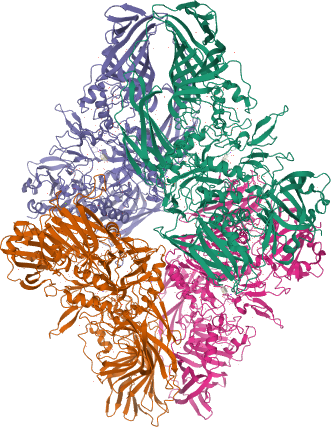
\includegraphics[height=5cm]{figures/5a1a_pdb.png}
            \caption*{\texttt{5a1a}}
        \end{subfigure}
        \hfill
        \begin{subfigure}[b]{0.42\linewidth}
            \centering
            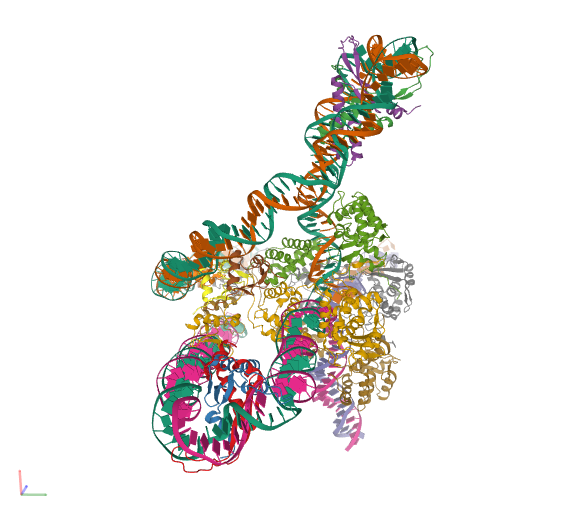
\includegraphics[height=5cm]{figures/5j0n_pdb.png}
            \caption*{\texttt{5j0n}}
        \end{subfigure}
        \caption{%
            Ground-truth atomic models: the $\beta$-galactosidase (\texttt{5a1a}), and the lambda excision HJ intermediate (\texttt{5j0n}).
            \todo{Show 5\AA\ density maps.}
        }\label{fig:pdb-proteins}
    \end{minipage}
    \hfill
    \begin{minipage}[b]{0.35\linewidth}
        \centering
        \begin{subfigure}[b]{0.49\linewidth}
            \centering
            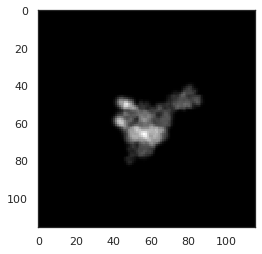
\includegraphics[width=0.8\linewidth]{figures/5j0n_noise0}
            \caption*{$\mathbf{P}_{\bth} \mathbf{x}$}
        \end{subfigure}
        \hfill
        \begin{subfigure}[b]{0.49\linewidth}
            \centering
            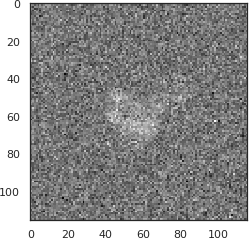
\includegraphics[width=0.8\linewidth]{figures/5j0n_noise16}
            \caption*{$\mathbf{P}_{\bth} \mathbf{x} + \mathbf{n}$}
    %, \; \mathbf{n} \sim \mathcal{N}(0, 16\mathbf{I})$}
        \end{subfigure}
        \\ \vspace{1em}
        \begin{subfigure}[b]{0.49\linewidth}
            \centering
            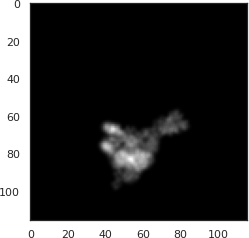
\includegraphics[width=0.8\linewidth]{figures/5j0n_translated}
            \caption*{$\mathbf{S}_{\mathbf{t}} \mathbf{P}_{\bth} \mathbf{x}$}
        \end{subfigure}
        \hfill
        \begin{subfigure}[b]{0.49\linewidth}
            \centering
            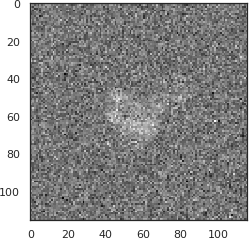
\includegraphics[width=0.8\linewidth]{figures/5j0n_noise16_translated}
            \caption*{$\mathbf{S}_{\mathbf{t}} \mathbf{P}_{\bth} \mathbf{x} + \mathbf{n}$}
        \end{subfigure}
        \caption{%
            Example projections of \texttt{5j0n}.
            % (a)~unperturbed, (b)~noisy, (c)~shifted, (d)~noisy and shifted.
        }\label{fig:different-projections}
    \end{minipage}
\end{figure}

\paragraph{Simulated projections.}
Using the ASTRA projector~\cite{van2015astra}, we generated $P=5,000$ synthetic projections of size ($275\times 275$) for \texttt{5a1a} and ($116\times 116$) for \texttt{5j0n}. 
\textcolor{red}{Jelena:} Orientations were obtained by uniformly sampling the Euler angles $\bth=(\theta_1,\theta_2,\theta_3) \in [0, \pi[ \times [0, \pi[ \subset [0, \pi[ \times [0, 2\pi[$ for \texttt{5j0n}, and $\bth=(\theta_1,\theta_2,\theta_3) \in [0, \pi[ \times [0, \pi[ \subset [0, \pi[ \times [0, 2\pi[$ for \texttt{5a1a}.
%\mdeff{Consistency: we used $\bth=(\theta_3,\theta_2,\theta_1)$ before. Which is better? Motivation for $(\theta_3,\theta_2,\theta_1)$ is that $\theta_1$ is the first rotation that is applied, through $\mathbf{R}_{\theta_1}$.} uniformly, and (ii) sampling uniformly on $\SO(3)$.
The \texttt{5j0n} complex being asymmetric, it was sufficient to only sample half  the $\mathbb{S}^2$ sphere parametrized by $(\theta_1,\theta_2)$.
%, the other half having equivalent projections symmetric to the center of this sphere.
Similarly, the $\beta$-galactosidase having D2 symmetry, %i.e., it is composed of four identical sub-units with two rotations of magnitude $\pi$ radians around the first axis followed by $\pi$ radians rotation around second axis, as illustrated and explained in~\cite{symmetry_in_protein,symmetry,scipion-em-github, rcsb-symmetry-view, EmpereurMot2019GeometricDO}.
%\mdeff{Do we need so many refs? Please check if they are all relevant.}
 we restricted the sampling to a quarter of the $\mathbb{S}^2$ sphere.
%\figref{different-projections} shows samples of the simulated projections.
%\mdeff{We should make it clear which 2 Euler angles parameterize $\mathbb{S}^2$, and which remaining one is to parameterize the full $\SO(3)$. Then we could be explicit and write something like we (uniformly?) sampled .}
Finally, as it is not possible to resolve chirality\footnote{An object is chiral if it cannot be superposed on its mirror image by any combination of translations or rotations.} (opposed projections being mirrored), we only trained on half coverage.
%Global orientation is lost by projecting, and chirality is lost by integrating.
%\mdeff{Not only a rotation, but an integration through $z_3$. (As opposed projections are mirrored, we cannot resolve chirality. Projecting looses global orientation, integrating looses chirality.)}
\todo{Write the range of angles we sampled from for \texttt{5j0n} and \texttt{5a1a}.}

We then perturbed the measurements with different levels of additive Gaussian noise~\cite{sorzano2004normalizing,shigematsu2013noise} and off-centering shifts. %, (iii) inclusion of the effects of the point-spread functions (PSF).
%\mdeff{Did we actually perform experiments with PSF?}
%The mathematical formulation of these three components is given in \eqnref{imaging-model}.
\figref{different-projections} displays samples of the simulated perturbations.
%\mdeff{Could we show the effect of the PSF?}

\begin{table}[ht!]
    \centering
    \begin{tabular}{lrrr}
        \toprule
        Dataset & Number of projections $P$ (\%) & Maximum number of pairs $P^2$ & Used number of pairs \\
        \midrule
        Training & 2512 (50\%) & 6,312,656 & 63,126 (1\%) \\
        Validation & 838 (17\%) & 701,406 & 7,014 (1\%) \\
        Test & 1650 (33\%) & 2,722,500 & all (sampled per batch) \\
        \bottomrule
    \end{tabular}
    \caption{%
        Split of $P=5000$ projections (for both \texttt{5j0n} and \texttt{5a1a}) in training, validation, and test sets.
        \todo{Fix the numbers.}
       % \mdeff{The number of pairs is given by $(P^2-P)/2$, not $P^2$ or $P^2-P$. Because pairs are made of distinct projections and order doesn't matter. Did we sample with those constraints?}
        %\banjac{thanks for remark, and I totally agree we need to use combinations of 2, however, I checked (and didn't notice before) that we use $P^2$ :(}
    }\label{tab:dataset}
\end{table}

% From projections to pairs and substes (which are used for distance learning and orientation recovery).
\paragraph{Splitting of Datasets.}
To train the SiameseNN, we used as input pairs of projections, and as output their respective quaternion distances (calculated from their orientations).
The number of possible projection pairs was $P^2 = 25 \times 10^6$. To generate the training, validation, and test datasets of projection pairs, we first split the $P$ projections into three distinct sets, and then generated the input datasets with disjoint projection sets (\tabref{dataset}); this was done to ensure that no projection would appear in projection pairs across the different training datasets.
%Splitting $P^2$ into the training, validation, and testing sets would mean that some of the projections appearing in pairs in the training dataset can appear in pairs in the other datasets.
%To ensure that the results generalize to unseen data, we split the projections $P$ (and not $P^2$) into training, validation, and testing projection sets.
%With these three projections sets we create disjoint projection pair datasets sets (column with $P^2$ values in \tabref{dataset}).
Note that we used only $1\%$ of the possible pairs due to limited available resources for training.
\todo{Explain why we do that.}
%\mdeff{So those pairs are sampled from $63,126$ pairs from the training dataset, rather than the $P^2$ possible pairs? If true, we should motivate somewhere why we limit our training dataset.}
\lau{Jelena:} The pairs for the training were sampled from $1\%$ of maximum number of training pairs $P_{\text{train}}^2$ ($63,126$ pairs) and validation was performed on $1\%$ of the maximum number of validation pairs $P_{\text{val}}^2$ ($27,225$ pairs). \lau{\textit{Jelena:} We restricted the size of our training and validation datasets due to Google Colaboratory\footnote{\lau{A hosted Jupyter notebook service from Google Research with resources that are not guaranteed and not unlimited.}} training time limit of 12 hours.} The training lasted from 2.6 hours to 9.3 hours on one GPU, depending on the available resources on \lau{the Google Colaboratory.} ADD INFORMATION ABOUT DISTRIBUTION BINNING, REASON FOR ONLY CONSIDERING A SUBSET. 
%\todo{Better explain why projections (and not pairs) must be separated in the various sets.}

Orientations were recovered through \eqnref{orientation-recovery} in a stochastic setting, with the loss function varying over the batches. The algorithm was deployed on the test set in \tabref{dataset} to ensure that it did not include any projection that was previously seen during the distance learning.

\paragraph{Optimization settings.}
We optimized \eqnref{distance-learning} with the RMSProp optimizer~\cite{tieleman2012rmsprop} and a learning rate of $10^{-3}$ for $150$ epochs. For a batch size of $256$, we have $247$ steps per epoch in training set and 28 steps per epoch in validation set (\tabref{dataset}).
%(i.e., $150 \times 63,126$ steps, \mdeff{correct?} \mdeff{Why didn't we sample for $x$ steps in the $6,312,656$ possible pairs? It seems arbitrary to artificially limit the pairs to $1\%$, and we'd see more combinations instead of seeing $150$ times the same pairs.}\banjac{we have 150 epochs and 63,126 pairs to go through in 1 epochs -> 63,126//265=247 steps per epoch through training data, and 28 steps for validation data}) on batches of $256$ pairs sampled from training sets .
We optimized \eqnref{orientation-recovery} with the Adam optimizer~\cite{kingma2014adam} and a learning rate of $0.5$ until convergence on batches of $256$ pairs sampled from the test sets (\tabref{dataset}).
%\todo{Figures~\ref{fig:5j0n-noise0-orientation-recovery},~\ref{fig:5j0n-noise16-orientation-recovery} and~\ref{fig:5a1a-noise0-orientation-recovery} show that more than $7000$ steps were used. We don't need to give a number, but could say something like we ran until convergence if that's how you did it. ;)}
%\mdeff{Jelena: when did you use the validation set? When the test?}
%\mdeff{With $7000$ steps we actually don't under-sample, as $7000 \times 256 > P^2-P)/2 \approx \num{350e3}$.}
We optimized \eqnref{orientation-recovery-error} with the FTRL optimizer~\cite{mcmahan2013ftrl} and a learning rate of $2$, a learning rate power of $-2$, a batch size of $256$ orientations. We reported the lowest of 6 runs (3 per value of $m$) of 300 steps each.
\todo{Jelena: check the settings, make sure they are used for all experiments, and add anything missing?}
\todo{Shortly mention the expected/average time to solve the different optimization problems. Then we don't discuss that anywhere else.}
% ($\sim$ 50 minutes in the best resource availability setting)

%%%%%%%%%%%%%%%%%%%%%%%%%%%%%%%%%%%%%%%%%%%%%%%%%%%%%%%%%%%%%%%%%%%%%%%%%%%%%%%%%%%%%%%

%\subsubsection{Robustness of Recovery to Additive Errors on the Relative Distances}

\subsection{Sensitivity of orientation recovery to errors in distance estimation}\label{sec:results:orientation-recovery:sensitivity}

%\mdeff{Story: (i) orientation recovery error is strongly linked to distance estimation error, (ii) recovery loss is a good proxy of mean recovery error.}
%\mdeff{Story: good distance estimation = good orientation recovery.}

\begin{wrapfigure}{r}{0.6\linewidth}
    \centering
    \begin{subfigure}[b]{0.48\linewidth}
        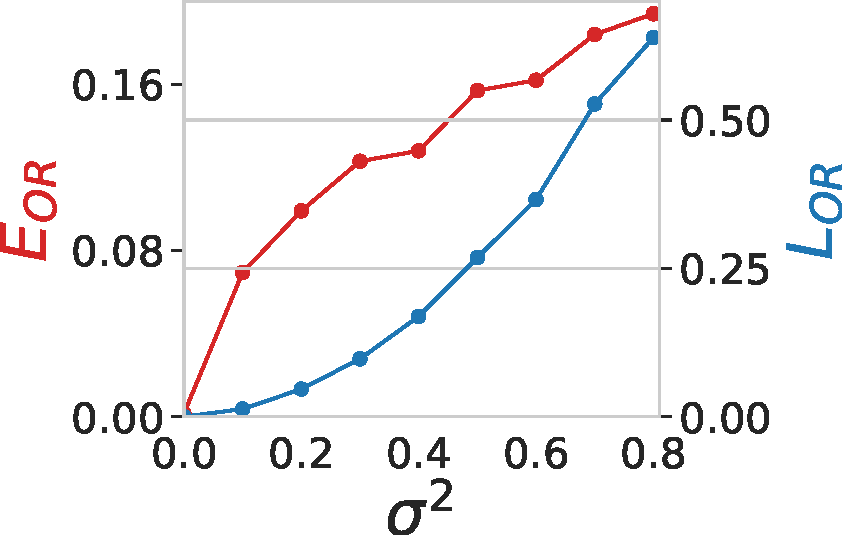
\includegraphics[height=3.3cm]{figures/5j0n_perfect_noisy_ar_aa}
        \caption{\texttt{5j0n}}
    \end{subfigure}
    \hfill
    \begin{subfigure}[b]{0.50\linewidth}
    \centering
        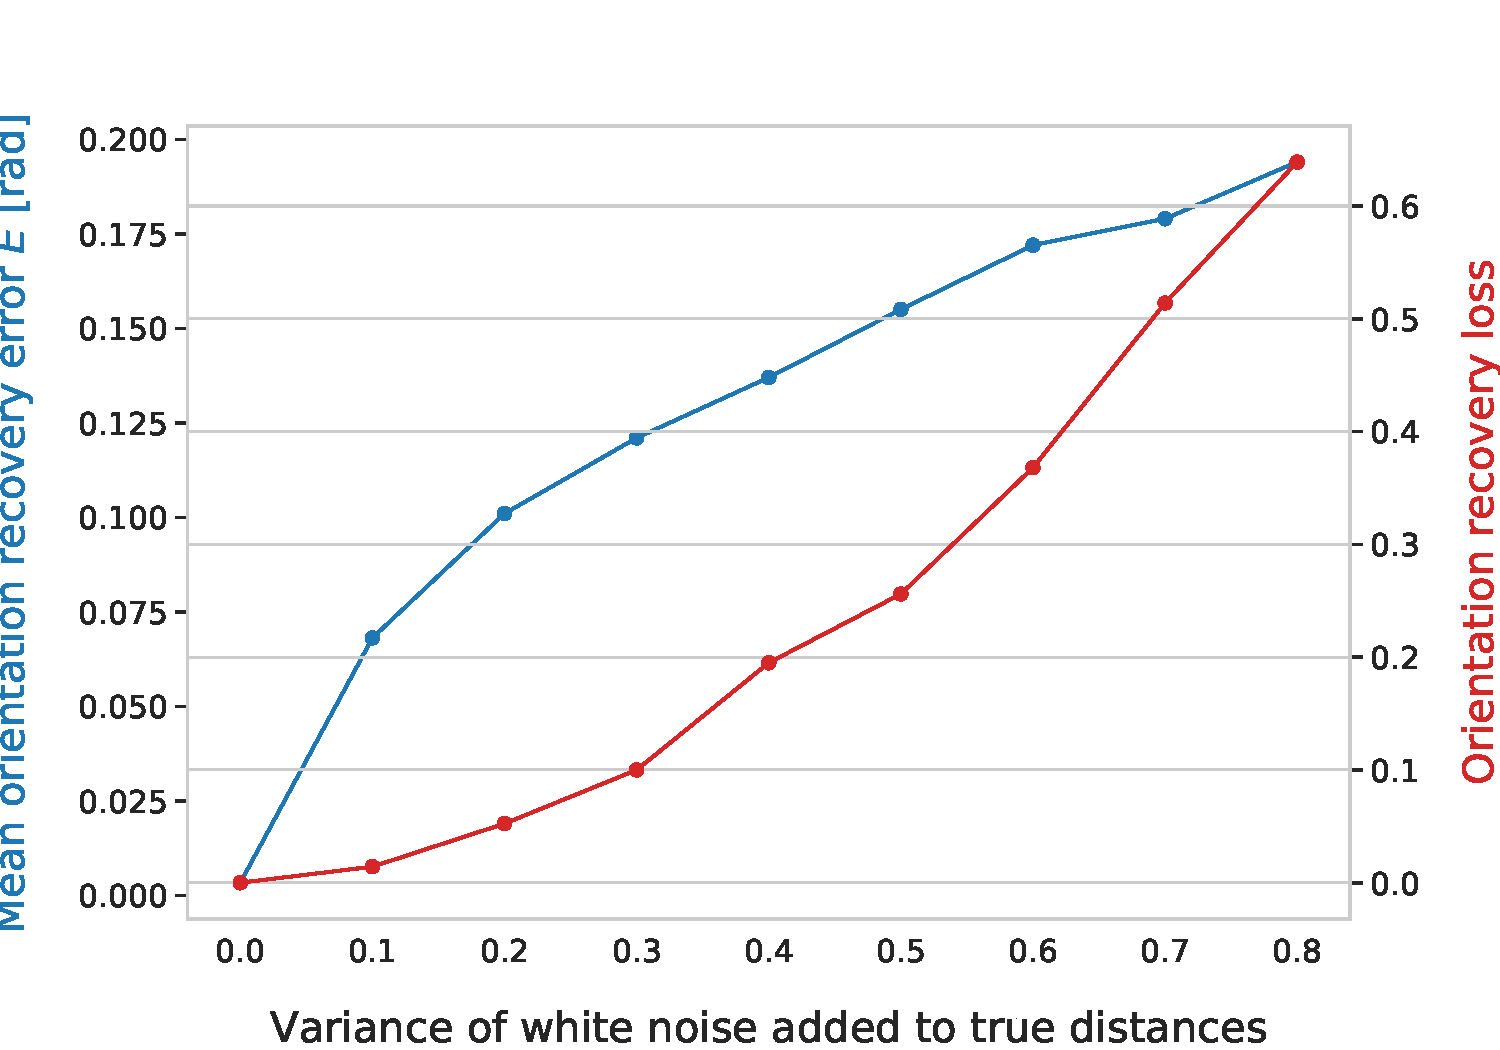
\includegraphics[height=3.3cm]{figures/5a1a_perfect_noisy_ar_aa}
        \caption{\texttt{5a1a}}
    \end{subfigure}
    \caption{
        The \textbf{mean orientation recovery error} $E_{OR}$ from \eqnref{orientation-recovery-error} is a monotonic function of the distance estimation error represented as a variance of white noise $\sigma^2$ added to the true distances.
        Better distance estimation leads to better orientation recovery.
        Moreover, the recovery loss $L_{OR}$ from \eqnref{orientation-recovery} is a good proxy for the recovery error $E_{OR}$, allowing us to assess recovery performance even without ground-truth orientations.
        \todo{Same axis ticks and sizes for both figures.}
    }\label{fig:perfect-with-noise-ar-aa}
\end{wrapfigure}

We first evaluated the feasibility of orientation recovery assuming that the exact quaternion distances between projection pairs were known.
Experiments confirmed that the method successfully recovers the orientation of every projection in this case (see \apxref{results:orientation-recovery:exact}).

We then evaluated the behaviour of~\eqnref{orientation-recovery} when the true relative distances were corrupted with an increasing level of additive Gaussian noise. More precisely, we perturbed the relative distances prior to the minimization with an error sampled from a Gaussian distribution with mean 0 and variances in $[0.0, 0.8]$.
The results are presented in \figref{perfect-with-noise-ar-aa} (red curve).
For all variances, the \textbf{mean orientation recovery error} $E_{OR}$ is reported in \figref{perfect-with-noise-ar-aa} (blue curve).

% \begin{figure}[ht!]
%     \centering
%     \begin{subfigure}[b]{0.48\linewidth}
%         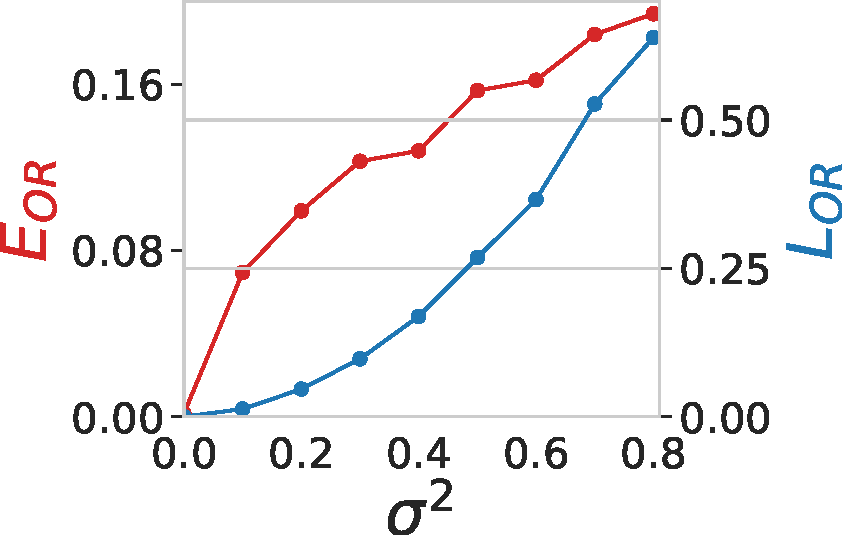
\includegraphics[height=3.5cm]{figures/5j0n_perfect_noisy_ar_aa}
%         \caption{\texttt{5j0n}}
%     \end{subfigure}
%     \hfill
%     \begin{subfigure}[b]{0.50\linewidth}
%     \centering
%         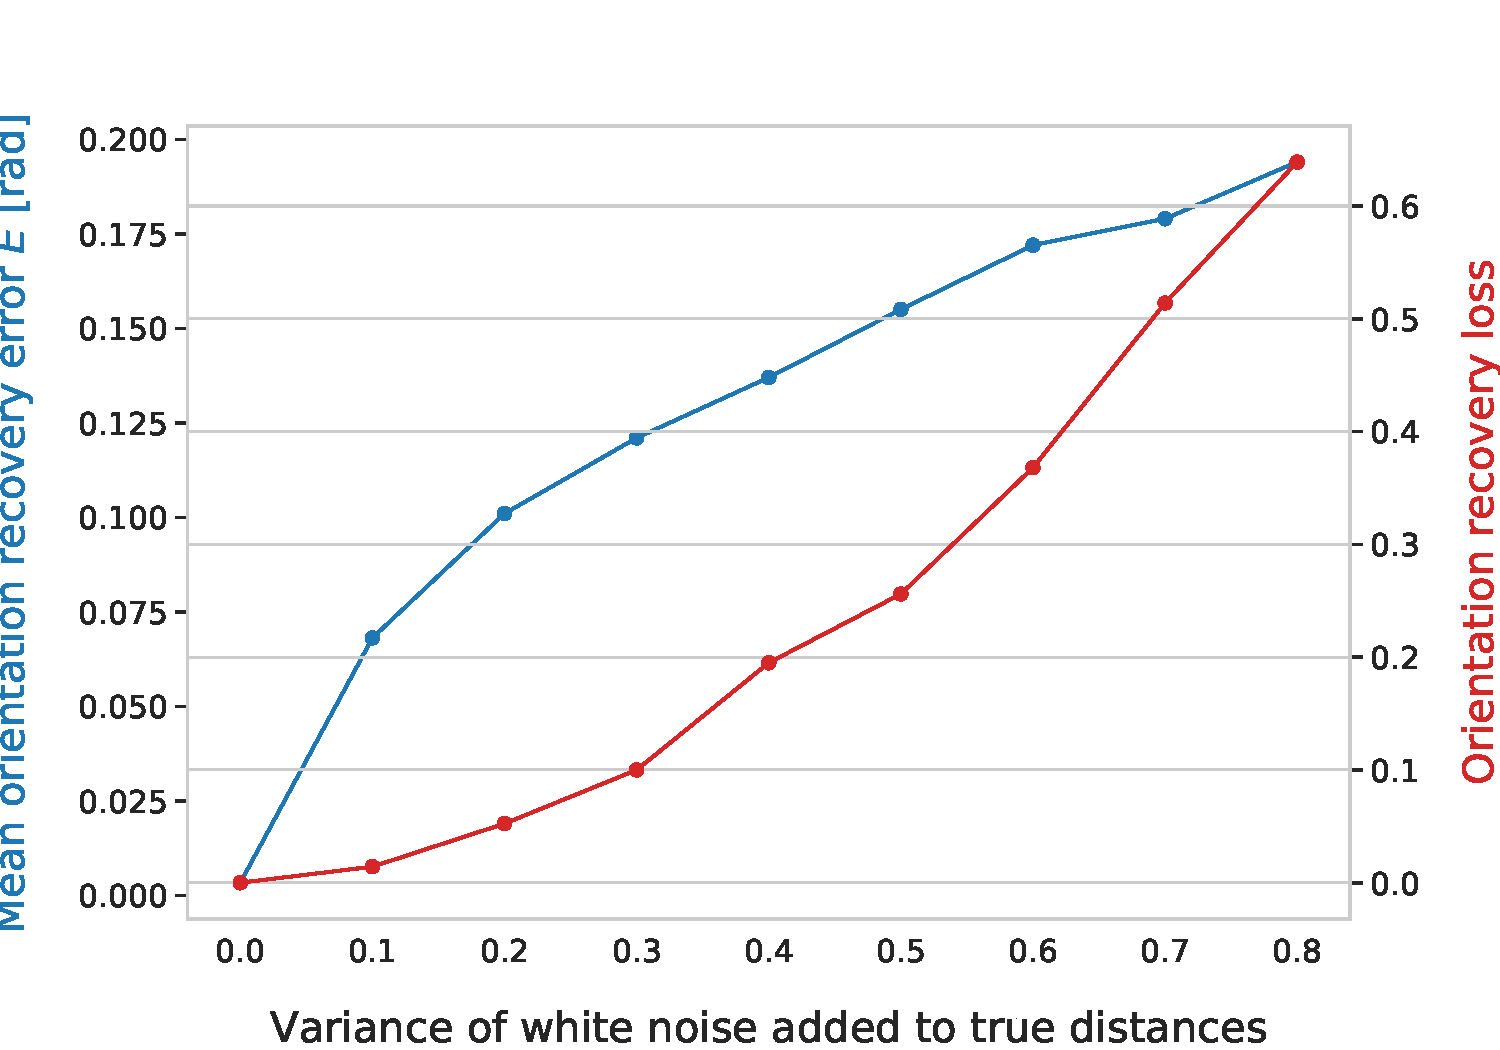
\includegraphics[height=3.5cm]{figures/5a1a_perfect_noisy_ar_aa}
%         \caption{\texttt{5a1a}}
%     \end{subfigure}
%     \caption{
%         The mean orientation recovery error $E_{OR}$ from \eqnref{orientation-recovery-error} is a monotonic function of the distance estimation error represented as a variance of white noise $\sigma^2$ added to the true distances.
%         Better distance estimation leads to better orientation recovery.
%         Moreover, the recovery loss $L_{OR}$ from \eqnref{orientation-recovery} is a good proxy for the recovery error $E_{OR}$, allowing us to assess recovery performance even without ground-truth orientations.
% }
%     \label{fig:perfect-with-noise-ar-aa}
% \end{figure}

These results demonstrate that the performance of orientation recovery~\eqnref{orientation-recovery} depends on the quality of the estimated distances, which advocates for a proper and extensive training of the SiameseNN in further stages of development.
Another interesting output of \figref{perfect-with-noise-ar-aa} is that it indicates that the \textbf{error of the orientation recovery} behaves as a monotonic function of its loss.
Hence, it suggests that the loss can be used as a good indicator of its performance, which has obvious practical implications for our future works on real data.
\mdeff{Obvious? I would specify: it allows to know how well the method worked when true distances aren't available.}

%%%%%%%%%%%%%%%%%%%%%%%%%%%%%%%%%%%%%%%%%%%%%%%%%%%%%%%%%%%%%%%%%%%%%%%%%%%%%%%%%%%%%%%

\subsection{Learned function for relative distance estimation }\label{sec:results:distance-estimation:learned}

%\mdeff{Story: learned distance $d_{ps}$ estimates $d_q$ with some variance but still underestimates larger distances.
%Again symmetric vs asymmetric.}

We evaluated how well our SiameseNN approximates the orientation distance $d_q$.
% ---parameterized as a SiameseNN and trained---
%s to learn a distance between projections $\widehat{d_p}(\p_i,\p_j)$
For comparison, we evaluated a baseline, the Euclidean distance $d_p(\p_i,\p_j) = \|\p_i, \p_j\|_2$, in \apxref{results:distance-estimation}.

\begin{figure}[ht!]
    \centering
    \begin{subfigure}[t]{0.45\linewidth}
        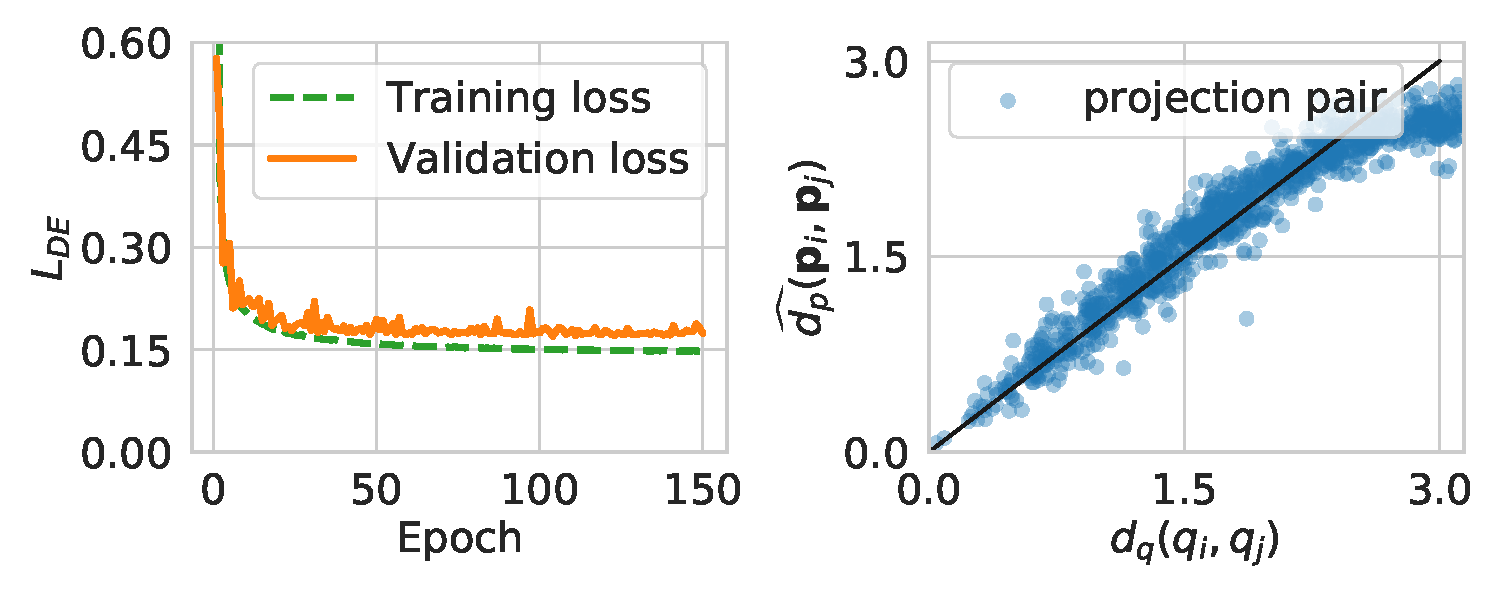
\includegraphics[height=3.3cm]{figures/de_loss_dPdQ_5j0n.pdf}
        \caption{\texttt{5j0n}}%
        \label{fig:losses-siamese-assym}
    \end{subfigure} \quad \quad
    \begin{subfigure}[t]{0.5\linewidth}
        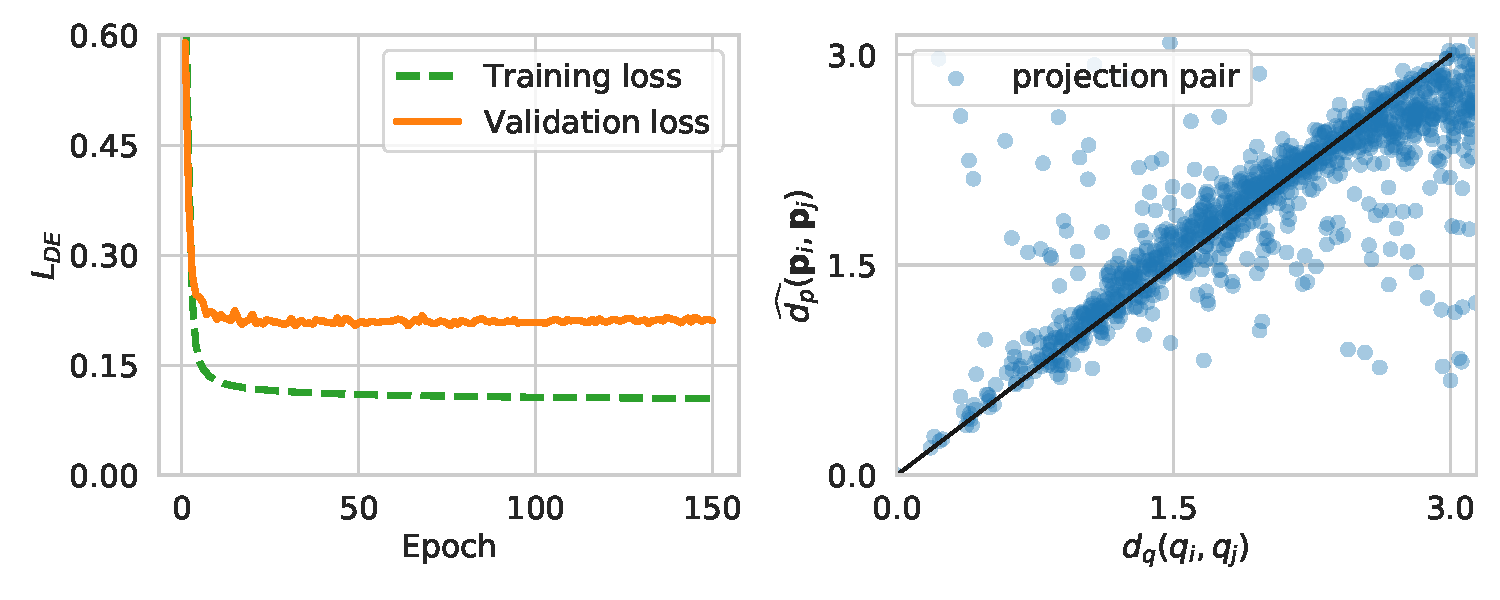
\includegraphics[height=3.3cm]{figures/de_loss_dPdQ_5a1a.pdf}
        \caption{\texttt{5a1a}}%
        \label{fig:losses-siamese-sym}
    \end{subfigure}
    \caption{%
        Distance learning loss $L_\text{DE}$ \eqnref{distance-learning} evaluated on the training and validation datasets during learning/training (on the left side respectively).
        Relationship between orientations' distance $d_q$ and estimated distance $d_p$ on the test dataset (on the right side respectively).
        We then fed the trained SiameseNN with $1,000$ pairs of projections randomly selected from the test dataset, and reported the $(d_q,\widehat{d_p})$ relationship of each pair.
        \todo{Arrange figure as a $2\times2$ grid. First row is the losses, second row the dP vs dQ. First column is \texttt{5j0n}, second column is \texttt{5a1a}. It'll be easier to compare the losses and dPdQ this way.}
        \todo{Consistency in legend: training and validation set.}
    }\label{fig:losses-siamese}
\end{figure}

\figref{losses-siamese}(a,b) shows how the distance learning loss converged during training.
Convergence was reached in about 50 epochs. %($50 x ? / 256$ steps).
%of the distance evolution of the training and validation losses for \texttt{5j0n} and \texttt{5a1a} are presented in and \figref{losses-siamese-sym}, respectively.
\todo{Values: $L_\text{DE} = ?$ for training/validation and \texttt{5j0n}/\texttt{5a1a}.}
While overfitting is low (the training and validation losses are close) for \texttt{5j0n}, it is larger for \texttt{5a1a}.
That's an indication that while we could train and learn a good distance on seen projections (training set), it doesn't generalize well to unseen projections (validation set).
That suggests that \texttt{5a1a} is harder than \texttt{5j0n}. \lau{Hypotheses: Some proteins have 3D density maps whose projections with close orientations are harder to distinguish from one another. Handling of symmetries could be done wrongly.}
\mdeff{Why is \texttt{5a1a} harder? Recurring theme (see 3.5).}
\mdeff{Here's an explanation by Jelena. Is it a good one? Let's discuss.}
\todo{This is most likely due to the symmetry of the protein (even though a quarter-sphere coverage was used.
%Indeed, its synthetic dataset may still contain pairs of projections that share the same $d_p$, yet differ in their $d_q$.
This  advocates for restricting to non-overlapping areas of $\SO(3)$ the sampling of the orientations used to generate the training dataset.
The latter would then only contain projection pairs with a linear $(d_q,d_p)$ relationship, which should ensure a successful training of the network.}
%\mdeff{I don't get this explanation. Do you mean that \texttt{5a1a} might have other symmetries than D2?}

\figref{losses-siamese}(c,d) shows the relation between the estimated distance $\widehat{d_p}$ and true distance $d_q$.
As expected, distances are better estimated for \texttt{5j0n} than \texttt{5a1a}.
While our learned distance function is a much better estimator than the Euclidean distance (compare \figref{losses-siamese}(c,d) with \figref{euclidean-not-robust}), they share one characteristic: both plateau and underestimate larger distances.
Though the issue is much less severe that with Euclidean distance.
\todo{Hypotheses: Because the true distances are upper-bounded by $\pi$? Training? Fixing a bit by sampling distances uniformly.}
Resolving this issue would ...
An alternative is to discard the larger distances and only rely on the estimation of local / short distances.
That would however require a force/loss/counter-balancing in \eqnref{orientation-recovery} to spread the orientations and prevent them to collapse to a single point.

% proxy distance
These results confirm that a SiameseNN is able to estimate differences in orientations from projections alone.
%Moreover, it clearly outperformed the Euclidean distance at doing so.
These preliminary results are encouraging; indeed, much has yet to be gained from improving upon the rather primitive SiameseNN architecture we are currently using.
Then train on more data (more pairs, data augmentation from imaging model \eqnref{imaging-model}, more proteins).
% Insist because that's a recurring theme of the paper.
Those will especially help when the task is more difficult, as for \texttt{5a1a}.
More data required to close the gap on \texttt{5a1a}, more powerful SiameseNN to push the losses down on both.
% Recurring theme.

%%%%%%%%%%%%%%%%%%%%%%%%%%%%%%%%%%%%%%%%%%%%%%%%%%%%%%%%%%%%%%%%%%%%%%%%%%%%%%%%%%%%%%%

\subsection{Sensitivity of distance learning to perturbations in the projections}\label{sec:results:distance-estimation:sensitivity}
%\subsection{Generalization of distance learning}
%\subsection{Generalizability/Abstractability of distance learning}

\mdeff{Shall we use ``noiseless projections'' or ``clean projections''?} \lau{Noiseless if space is not an issue.}

%\mdeff{Story: learned distance is minimally sensible to perturbations (additive noise, translation, PSF) because we can train it to ignore irrelevant information.
%Thanks again to good model of cryo-EM imaging.}
%\mdeff{Better word? (perturbations, corruptions, quality, non-ideal)}

% Intro and shift.
We desire to estimate distances that are invariant to perturbations in the projections---specified in~\eqnref{imaging-model}.
As discussed in \secref{method:distance-learning}, the convolutional architecture of the SiameseNN should be shift invariant.
\figref{results:distance-estimation:shift} indeed shows that learning distances (and hence recovering orientations) is insensible to shifts in projections.

% Noise.
As we cannot---or do not (yet) know how to---build noise invariance into the architecture, we trained the SiameseNN on noisy datasets and evaluated whether it could learn to ignore noise as being irrelevant information.
% brute force vs principled engineering
\figref{results:distance-estimation:noise} shows a mean orientation recovery error of $E_\text{OR} \approx 0.16$ radians ($\approx 9\degree$) for noiseless projections and $E_\text{OR} \approx 0.42$ radians ($\approx 24\degree$) for a more realistic noise variance of $\sigma^2=16$.
\mdeff{How good is that?}\banjac{To be discussed tomorrow}\lau{Reasonable first guess, room for improvement.}
While a naive distance function (like an Euclidean distance) would be tremendously sensitive to noise, the SiameseNN mostly learned to discard it.
Moreover, overfitting (i.e., the growing gap between the validation and trainig losses) indicates that more training data will further decrease the SiameseNN's sensitivity to noise.

% PSF and conclusion.
We didn't evaluate sensitivity to the PSF but expect a similar behavior.
%While we would ideally want the NN architecture to be engineered to ignore irrelevant information, that is not always possible.
%We know how to do it for shifts, not noise or PSF.

We observe that the estimation of more accurate distances (a smaller $L_\text{DE}$) leads to the recovery of more accurate orientations (a smaller $L_\text{OR}$ and $E_\text{OR}$).
Moreover, we observe again (\secref{results:orientation-recovery:sensitivity}) that an higher recovery loss $L_\text{OR}$ induces an higher error $E_\text{OR}$.

%\subsection{Estimating distances on unseen proteins}

As the SiameseNN will ultimately be trained on known proteins and used to estimate distances on unknown proteins to be imaged,
%we also desire our learned distance function to generalize/transfer across density maps $\x$.
we also desire our learned distance function to generalize to unseen proteins.
The distance function $\widehat{d_p}$ must abstract the protein (in the same way it must abstract shifts, noise, or PSFs to generalize to unseen projections).
We attempted to recover the orientations of noiseless projections from \texttt{5j0n} while we had trained the SiameseNN on noiseless projections of four other proteins (\texttt{5nvu}~\cite{5nvu_pdb}, \texttt{5nvs}~\cite{5nvs_pdb}, \texttt{6mem}~\cite{6mem_pdb}, \texttt{6o1o}~\cite{6o1o_pdb} \todo{should be the same ``kind'' of refs as the ones used in 3.1 for \texttt{5j0n} and \texttt{5a1a}}, which have the same type of symmetry as \texttt{5j0n}).
In this experiment, we generated $1,000$ projections per protein.
The \todo{percentage?} of projections split in the training, validation, and test sets is the same as in \tabref{dataset}.
Then, four proteins are used in the training and validation set to ensure the robustness to the unseen protein \texttt{5j0n} used in the testing set.
We obtained a recovery loss of $L_\text{OR} = 0.0352$ \mdeff{Could we also have $E_\text{OR}$? It's easier to understand and compare.}\banjac{I fully agree, however, I already mentioned that I wasn't able to align the orientations even though the $L_{OR}$ was very good. Looking at the estimation and GT in rotation space, it is visible we have some kind of transformation between these two (transformation similar to one we found the flip is causing, but it is not the flip)},
\mdeff{Right, thanks for explaining again. We should probably talk about that issue somewhere. An Appendix? Do we have examples when it worked and when it didn't?}
% Jelena: Angle recovery is good but it is unable to align. Probably missing something as expected as a flip discovered at the beginning of the project.
to be compared with $L_\text{OR} \approx 0.11$ when the SiameseNN was trained on \texttt{5j0n} alone.
While performance is somewhat degraded, we conclude that it is possible to use a learned distance function on unseen proteins.

\begin{figure}[ht!]
    \centering
    \begin{subfigure}[t]{0.47\linewidth}
        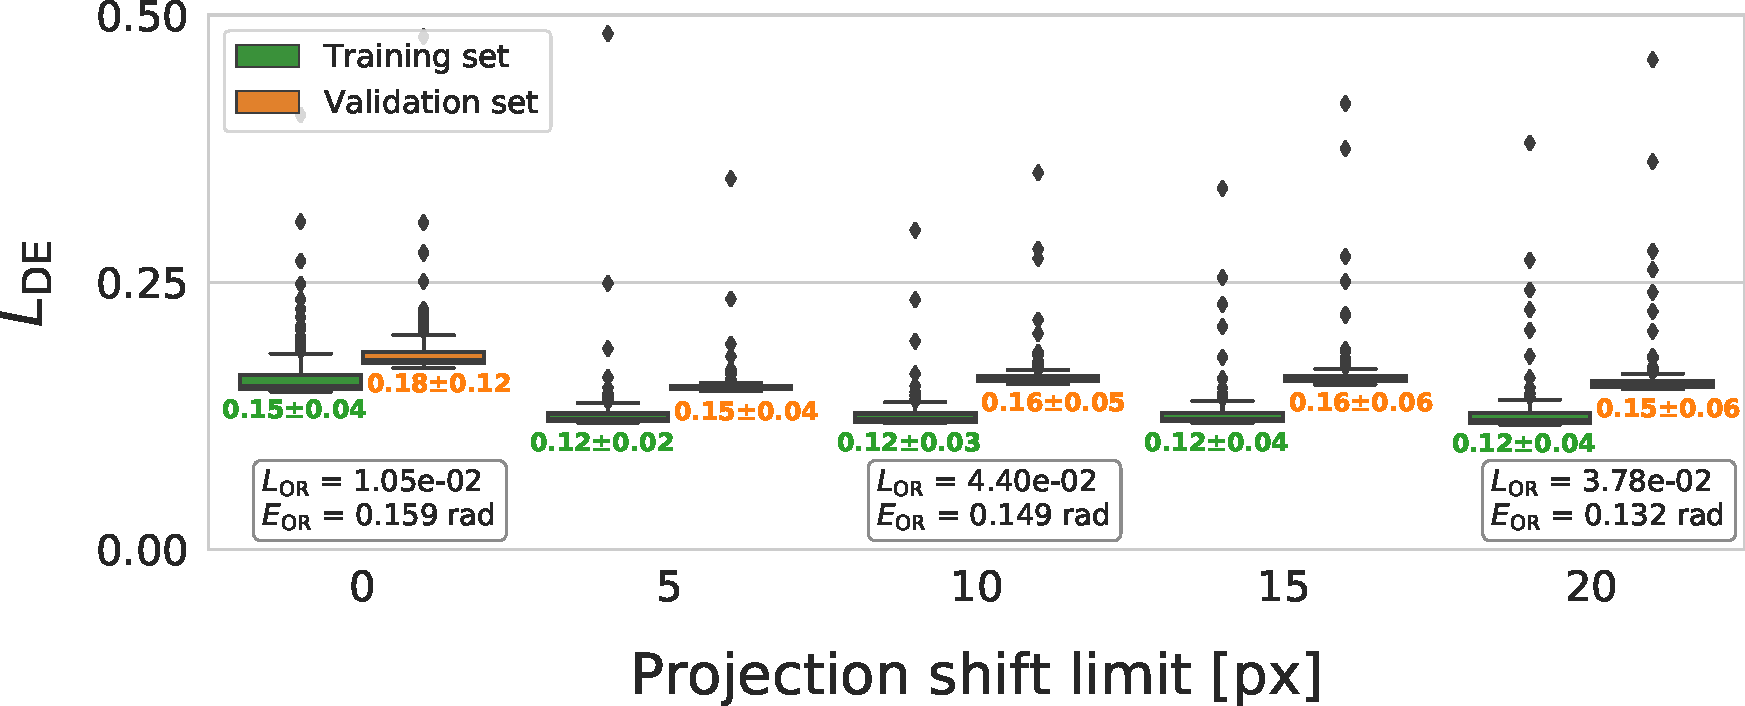
\includegraphics[width=\linewidth]{figures/de_translation_nums}
        \caption{%
            Learning from shifted projections $\{ \mathbf{S}_{\mathbf{t}_i} \mathbf{P}_{\bth_i} \mathbf{x} \}$, with translations $t_{i_1}$ and $t_{i_2}$ sampled from a triangular distribution with mean 0 and of increasing limits.
            Learning is not harder as projections get shifted farther, because shift invariance is built into the convolutional architecture of $\mathcal{G}_w$.
    }\label{fig:results:distance-estimation:shift}
    \end{subfigure}
    \hfill
    \begin{subfigure}[t]{0.47\linewidth}
        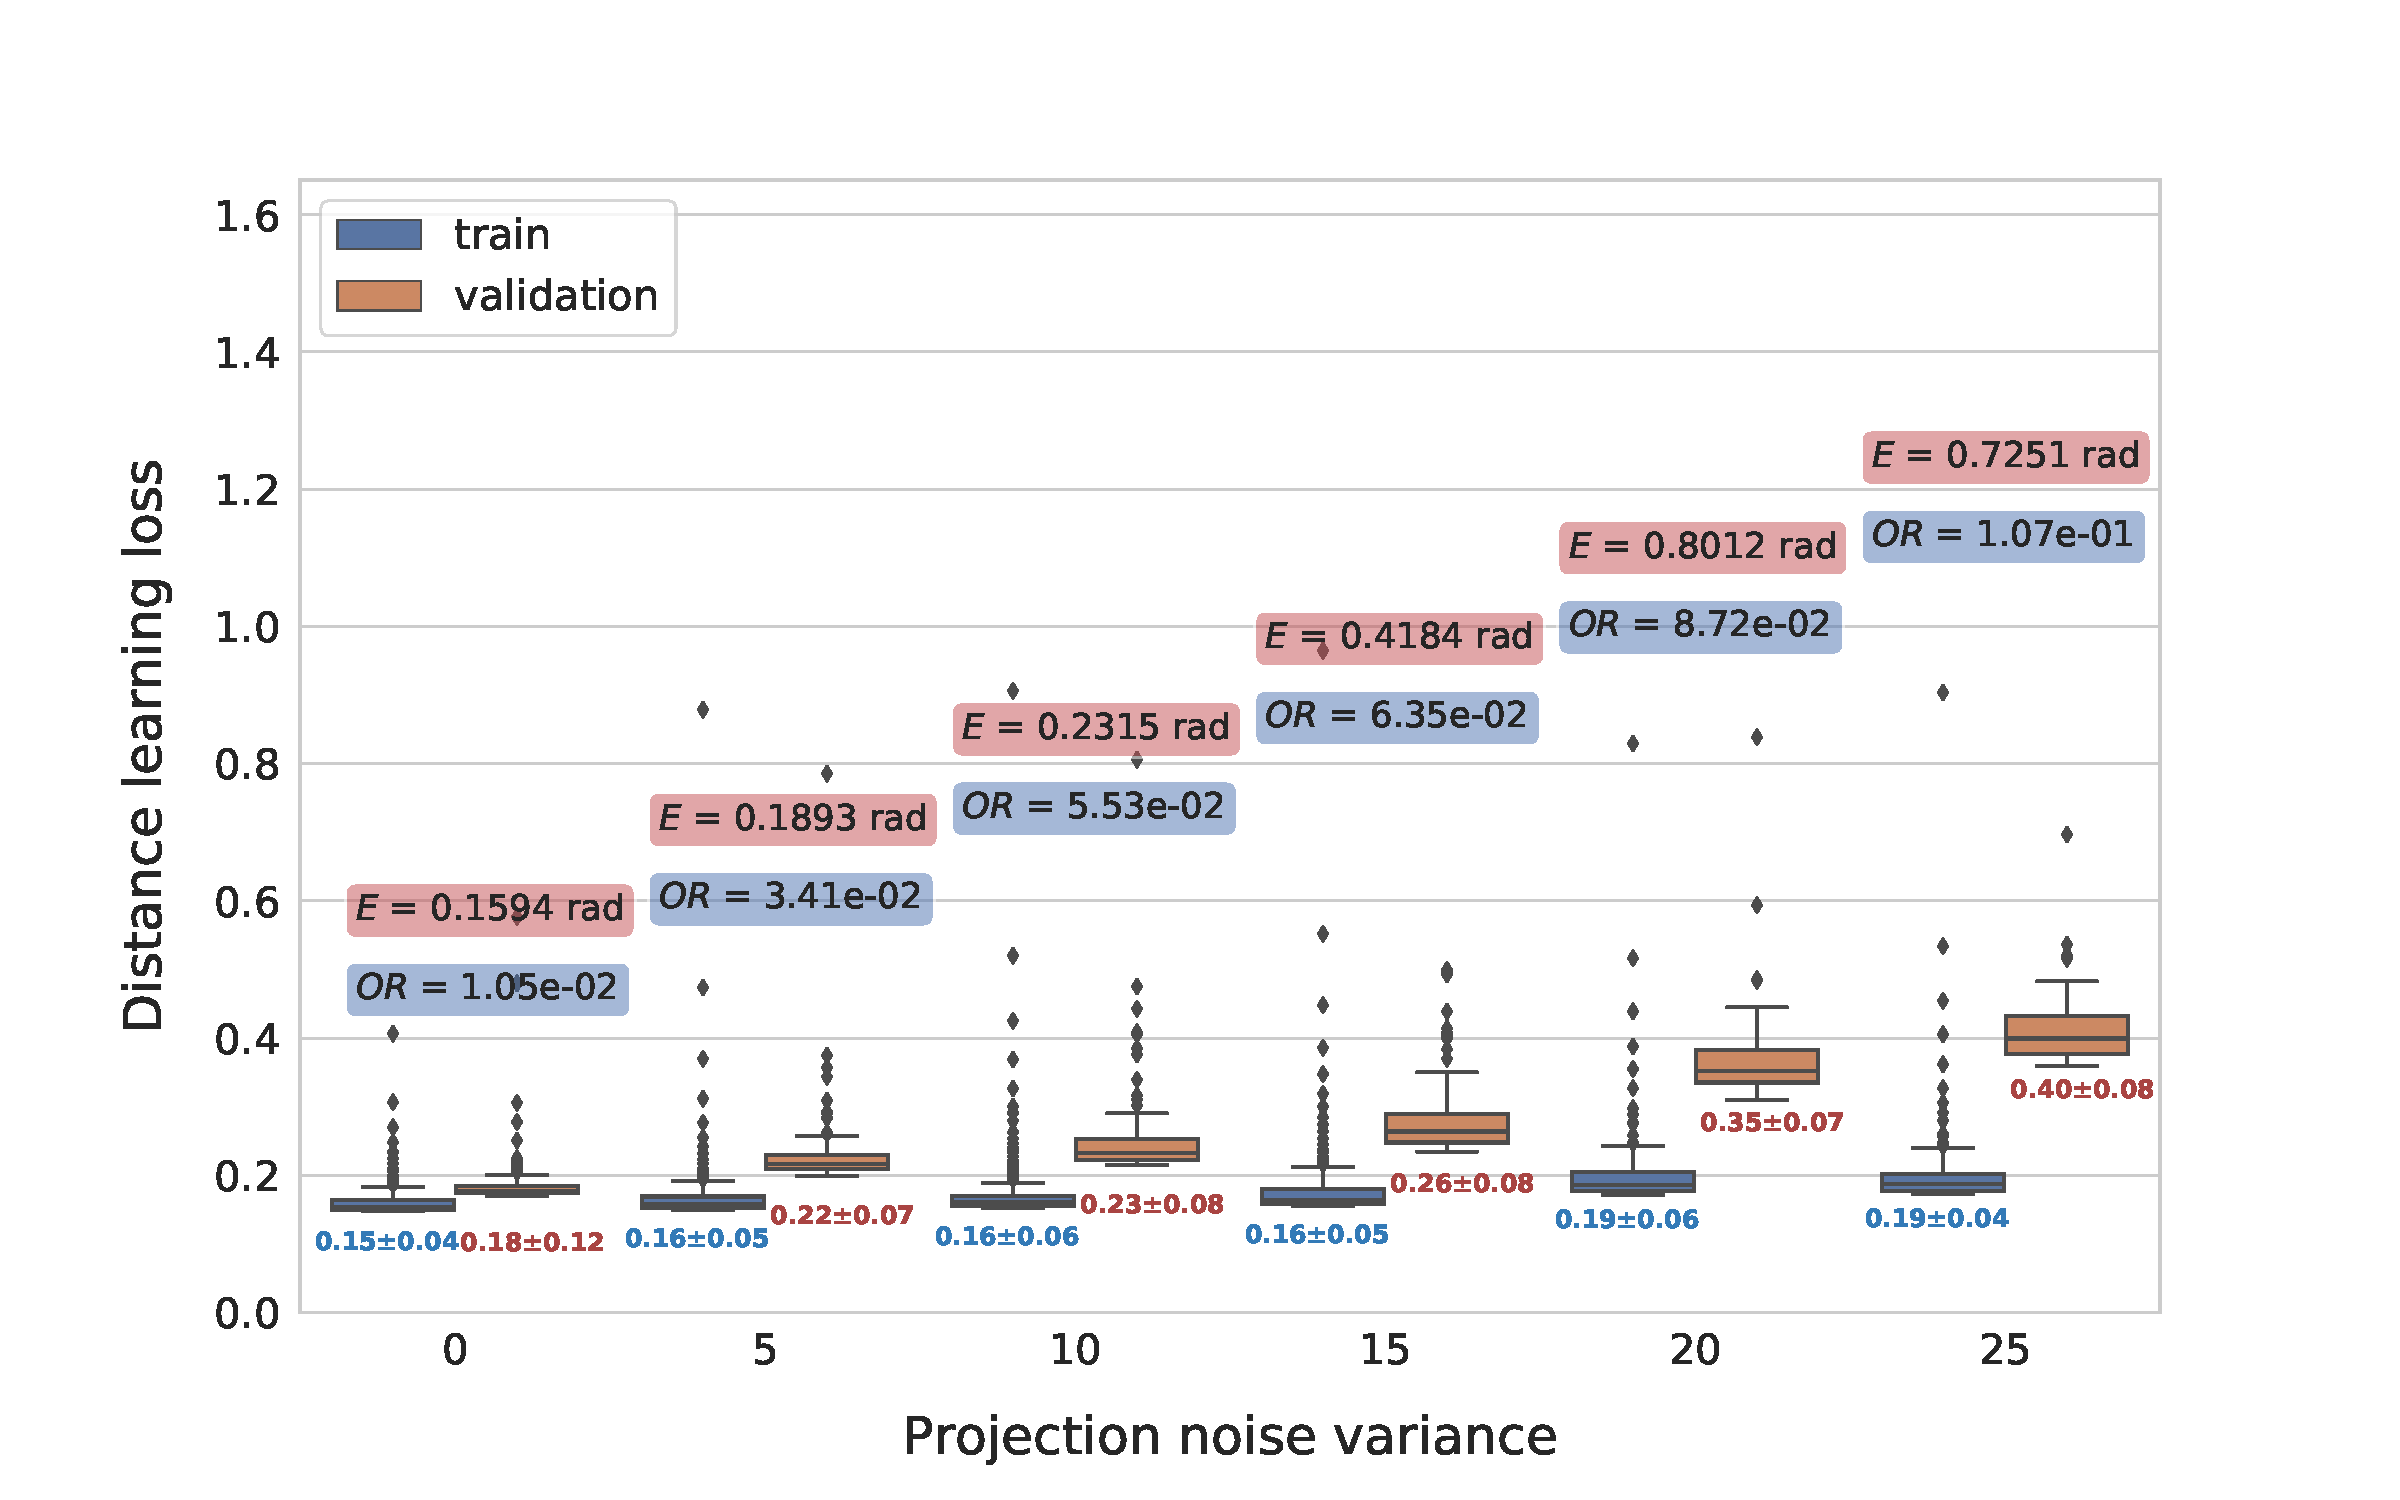
\includegraphics[width=\linewidth]{figures/de_noises_nums}
        \caption{%
            Learning from noisy projections $\{ \mathbf{P}_{\bth_i} \mathbf{x} + \mathbf{n} \}$, with white noise $\mathbf{n} \sim \mathcal{N}(0, \sigma^2\mathbf{I})$ of increasing variance $\sigma^2$.
            Learning is harder as projections get noisier, because noise invariance is not built into the architecture of $\mathcal{G}_w$.
        }\label{fig:results:distance-estimation:noise}
    \end{subfigure}
    \caption{%
        Sensitivity of distance learning to perturbations in the projections of \texttt{5j0n}.
        The box plots show the distance learning loss $L_\text{DE}$ per epoch \eqnref{distance-learning} on the training (blue) and validation (red) sets.
        %\mdeff{Numbers are per pair or per batch of 256 pairs?}
        Boxes show the orientation recovery loss $L_\text{OR}$ \eqnref{orientation-recovery} and error $E_\text{OR}$ \eqnref{orientation-recovery-error}.
        %\mdeff{It's confusing that red and blue are used for both train vs validation and $E_\text{OR}$ vs $L_\text{OR}$. I don't think we need colors for $E_\text{OR}$ and $L_\text{OR}$. They could both be in the same black box.}
        %\todo{Legend consistency: train -> training set, validation -> validation set.}
        %\todo{Add $L_\text{DE}$ to the y-axis legend.}
        %\todo{Add $\sigma^2$ to the x-axis legend of (b).}
    }
\end{figure}

%%%%%%%%%%%%%%%%%%%%%%%%%%%%%%%%%%%%%%%%%%%%%%%%%%%%%%%%%%%%%%%%%%%%%%%%%%%%%%%%%%%%%%%

\subsection{Orientation recovery and density reconstruction from estimated distances}\label{sec:results:orientation-recovery:reconstruction}
%\subsection{Density reconstruction from recovered orientations}

\todo{
\begin{itemize}
    \item \mdeff{Should we call it Density reconstruction from recovered orientations?}
    %\item Make the plots in Figures~\ref{fig:5j0n-noise0-orientation-recovery},~\ref{fig:5j0n-noise16-orientation-recovery}, and~\ref{fig:5a1a-noise0-orientation-recovery} flatter and remove \texttt{width=linewidth} (which deforms the figure).
    %\item Add $L_\text{OR}=...$ and $E_\text{OR}=...$ in the boxes of Figures~\ref{fig:5j0n-noise0-orientation-recovery},~\ref{fig:5j0n-noise16-orientation-recovery}, and~\ref{fig:5a1a-noise0-orientation-recovery}.
    \item Would be nice to know $L_\text{DE}$ for the three cases. \banjac{On the test set?}
    %\item ``With total of $1,650$ projections in the test dataset, we were able to reconstruct the protein.'' \mdeff{But \tabref{dataset} says 838 for test. Was it validation data?} \banjac{Great notice!! The table was wrong, I fixed it. In the code I was printing in different order so I mixed it.}
    \item \mdeff{Training set for distance learning and validation/test set for orientation recovery should have been made clear in 3.1.} \banjac{Actually, train and validation sets are used in distance learning, and test set was only used for dPdQ plot, orientation recovery (and alignment)}
\end{itemize}
}

As a proof-of-concept, we attempted to solve the inverse problem posed by \eqnref{imaging-model}.
We reconstructed density maps $\widehat{\x}$ from sets of projections $\{ \p_i \}$ and their orientations $\{ \widehat{q_i} \}$ as recovered by our method.
%We ran the full pipeline---distance estimation, orientation recovery, and protein reconstruction---to validate our method.
%The orientation recovery from estimated distances represents a full pipeline needed to reconstruct the protein from a given set of projections.
Note that we only trained the SiameseNN \eqnref{distance-learning} on projections from the protein (and noise level) we attempted to reconstruct from.
For best performance, it should be trained on multiple proteins, levels of noise, PSFs, etc.

\lau{Smooth this paragraph:}To understand the effect of miss-recovered orientations, we reconstructed the density maps from both the recovered orientations $\{ \widehat{q_i} \}$ and the true orientations $\{ q_i \}$ along which the projections $\{ \p_i \}$ were acquired.
The density maps were reconstructed by the ASTRA toolbox.
\todo{Using the ASTRA toolbox, we generated orientation vectors based on angles which we fed into projection 3D geometry in ASTRA.}
\todo{Make clearer. Are there enough details?}
\mdeff{Laurène, could you write something about how ASTRA is a naive reconstruction method (compared to the SOTA discussed in the intro), and that we did it only to get a crude idea? Or something along those lines. ;)} \lau{Not naïve actually, just direct hence less robust. I think it's a good idea to write this, i.e. that the quality of reconstruction is likely to improve with a more robust algorithm, but I'm wondering if we should not put that in the discussion/conclusion.}
For an unknown reason, we had to align the recovered orientations with \eqnref{orientation-recovery-error} before feeding them to ASTRA.
\todo{More details. What happened otherwise? We want to say it's an ASTRA issue not something with our method.} \lau{Yeah but I wouldn't blame ASTRA at all, it's dangerous territory. There is just an engineering problem we haven't been able to solve, let's not blame well-know, widely-used existing packages out there if possible.}

\begin{figure}[t]
    \centering
    \begin{subfigure}[b]{0.44\linewidth}
        \centering
        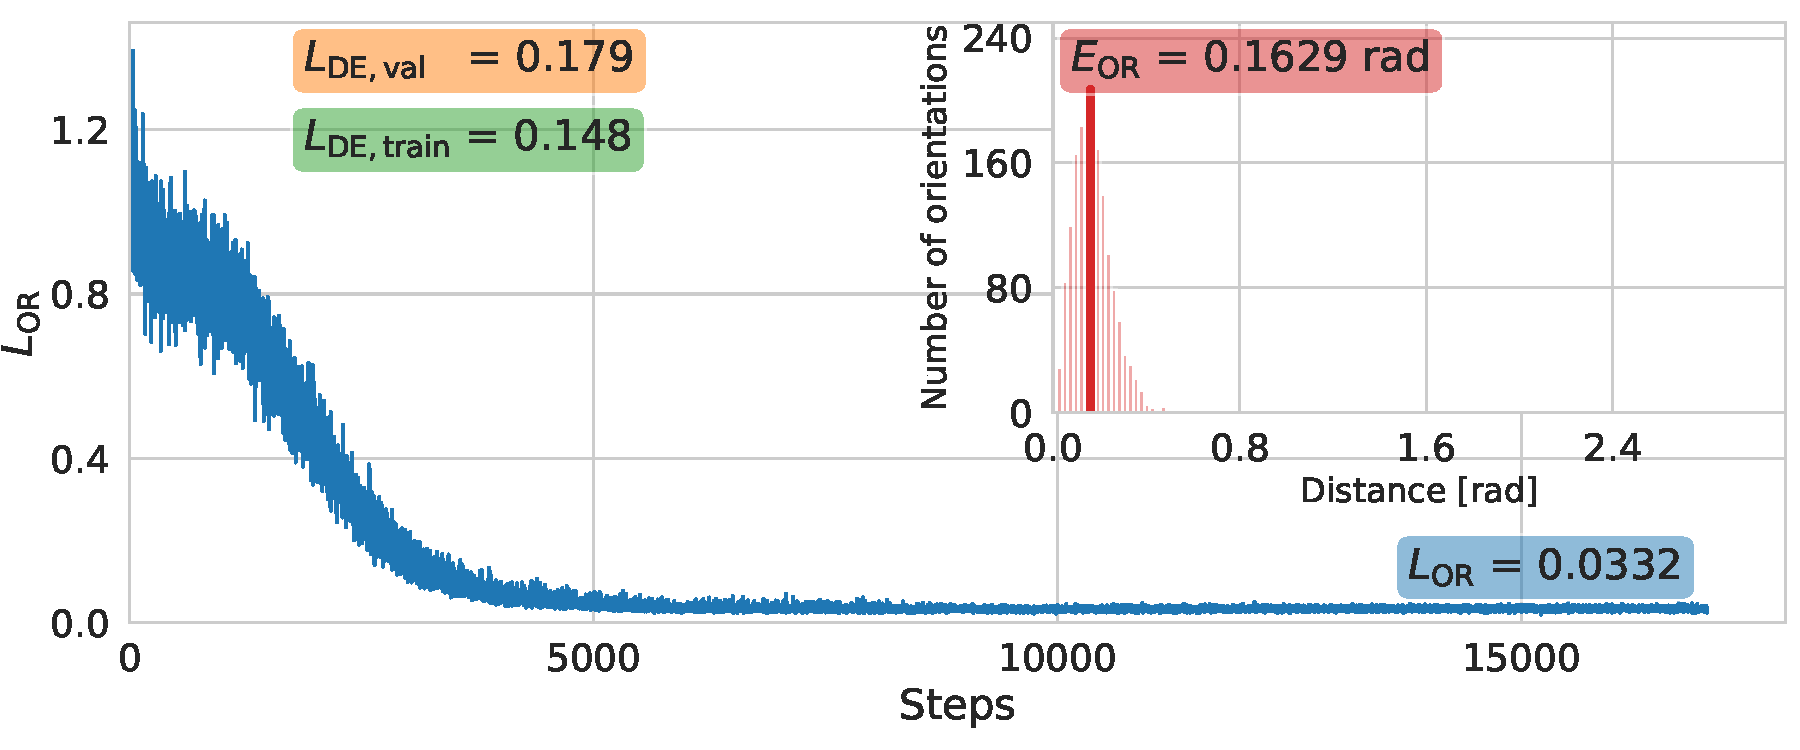
\includegraphics[height=8em]{figures/5j0n_noise0_ar_aa}
        \caption{Recovered $\{ \widehat{q_i} \}$ from $\{ \p_i = \mathbf{P}_{\bth_i} \x \}$, $\x$ from \texttt{5j0n}.}%
        \label{fig:5j0n-noise0-orientation-recovery}
    \end{subfigure}
    \hfill
    \begin{subfigure}[b]{0.26\linewidth}
        \centering
        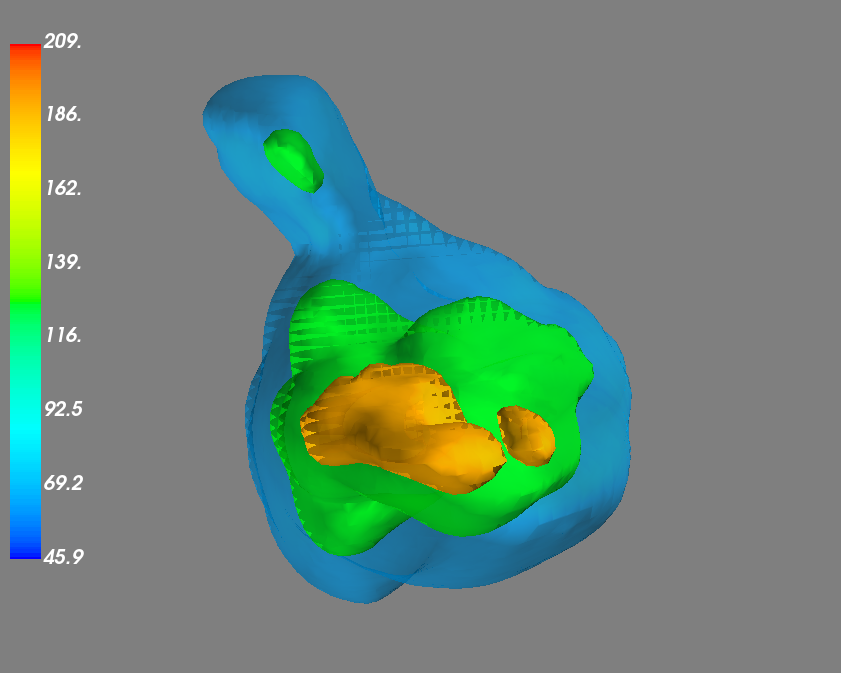
\includegraphics[height=8em]{figures/5j0n_reconstruction_noise0}
        \caption{Reconstructed $\widehat{\x}$ from $\{ \p_i, \widehat{q_i} \}$.}%
        \label{fig:5j0n-noise0-reconstruction-recovered}
    \end{subfigure}
    \hfill
    \begin{subfigure}[b]{0.26\linewidth}
        \centering
        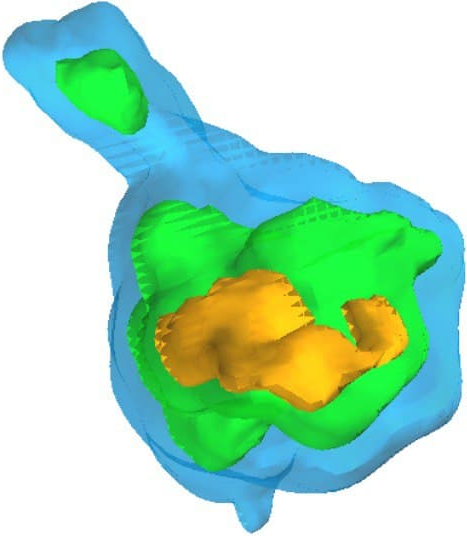
\includegraphics[height=8em]{figures/5j0n_reconstruction_GT}
        \caption{Reconstructed $\widehat{\x}$ from $\{ \p_i, q_i \}$.}%
        \label{fig:5j0n-noise0-reconstruction-true}
    \end{subfigure}
    \\ \vspace{1em}
    \begin{subfigure}[b]{0.44\linewidth}
        \centering
        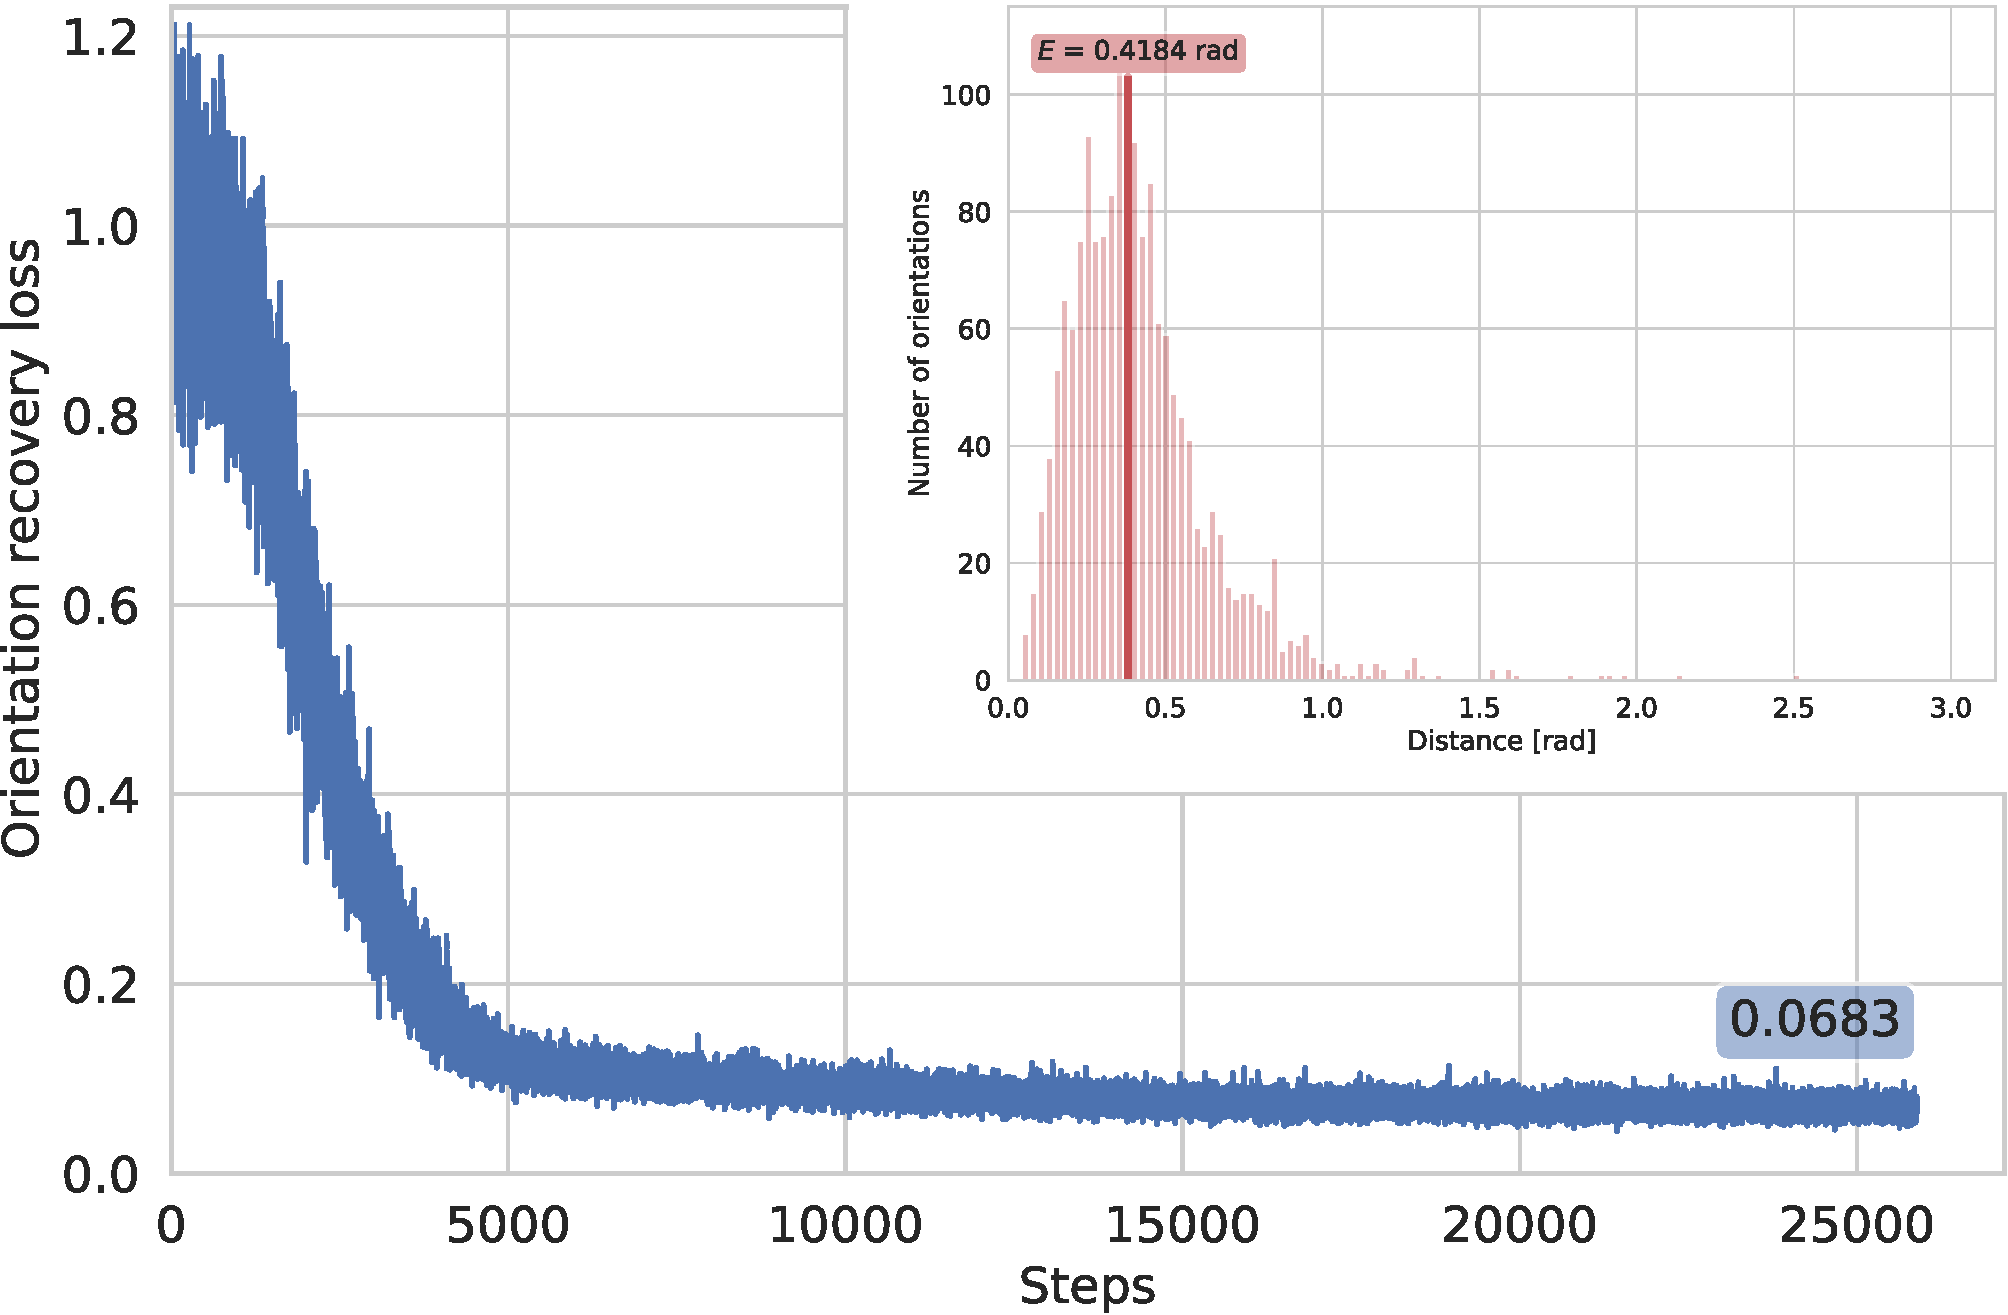
\includegraphics[height=8em]{figures/5j0n_noise16_ar_aa}
        \caption{Recovered $\{ \widehat{q_i} \}$ from $\{ \p_i = \mathbf{P}_{\bth_i} \x + \mathbf{n} \}$, $\x$ from \texttt{5j0n}.}%
        \label{fig:5j0n-noise16-orientation-recovery}
    \end{subfigure}
    \hfill
    \begin{subfigure}[b]{0.26\linewidth}
        \centering
        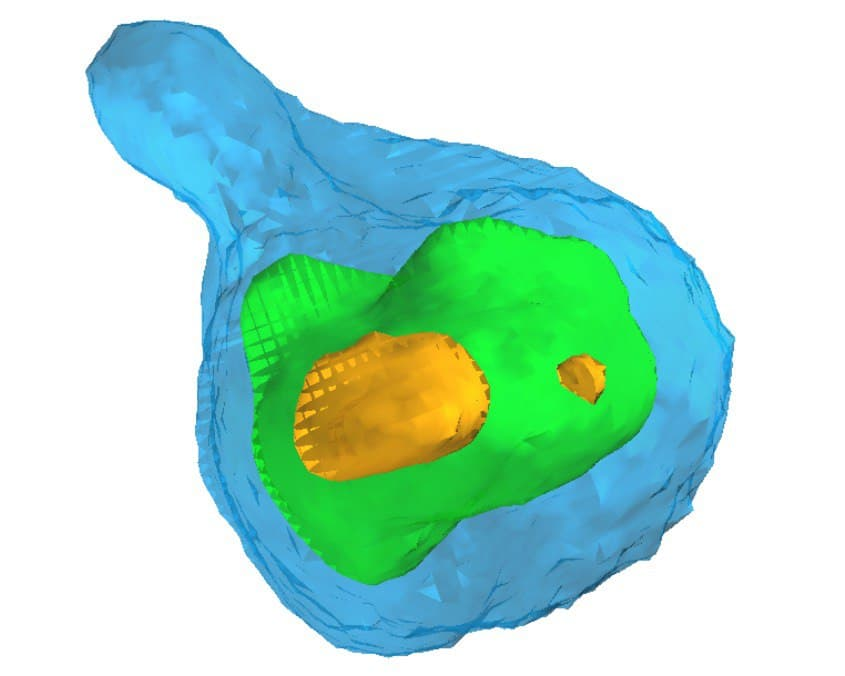
\includegraphics[height=8em]{figures/5j0n_reconstruction_noise16}
        \caption{Reconstructed $\widehat{\x}$ from $\{ \p_i, \widehat{q_i} \}$.}%
        \label{fig:5j0n-noise16-reconstruction-recovered}
    \end{subfigure}
    \hfill
    \begin{subfigure}[b]{0.26\linewidth}
        \centering
        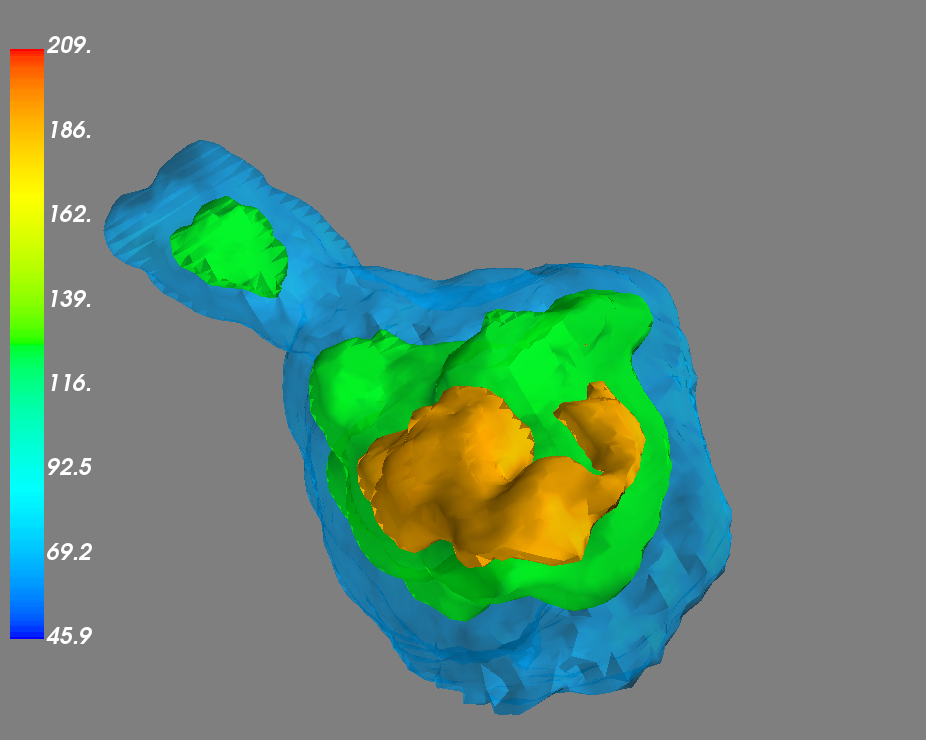
\includegraphics[height=8em]{figures/5j0n_reconstruction_GT_noise16}
        \caption{Reconstructed $\widehat{\x}$ from $\{ \p_i, q_i \}$.}%
        \label{fig:5j0n-noise16-reconstruction-true}
    \end{subfigure}
    \\ \vspace{1em}
    \begin{subfigure}[b]{0.44\linewidth}
        \centering
        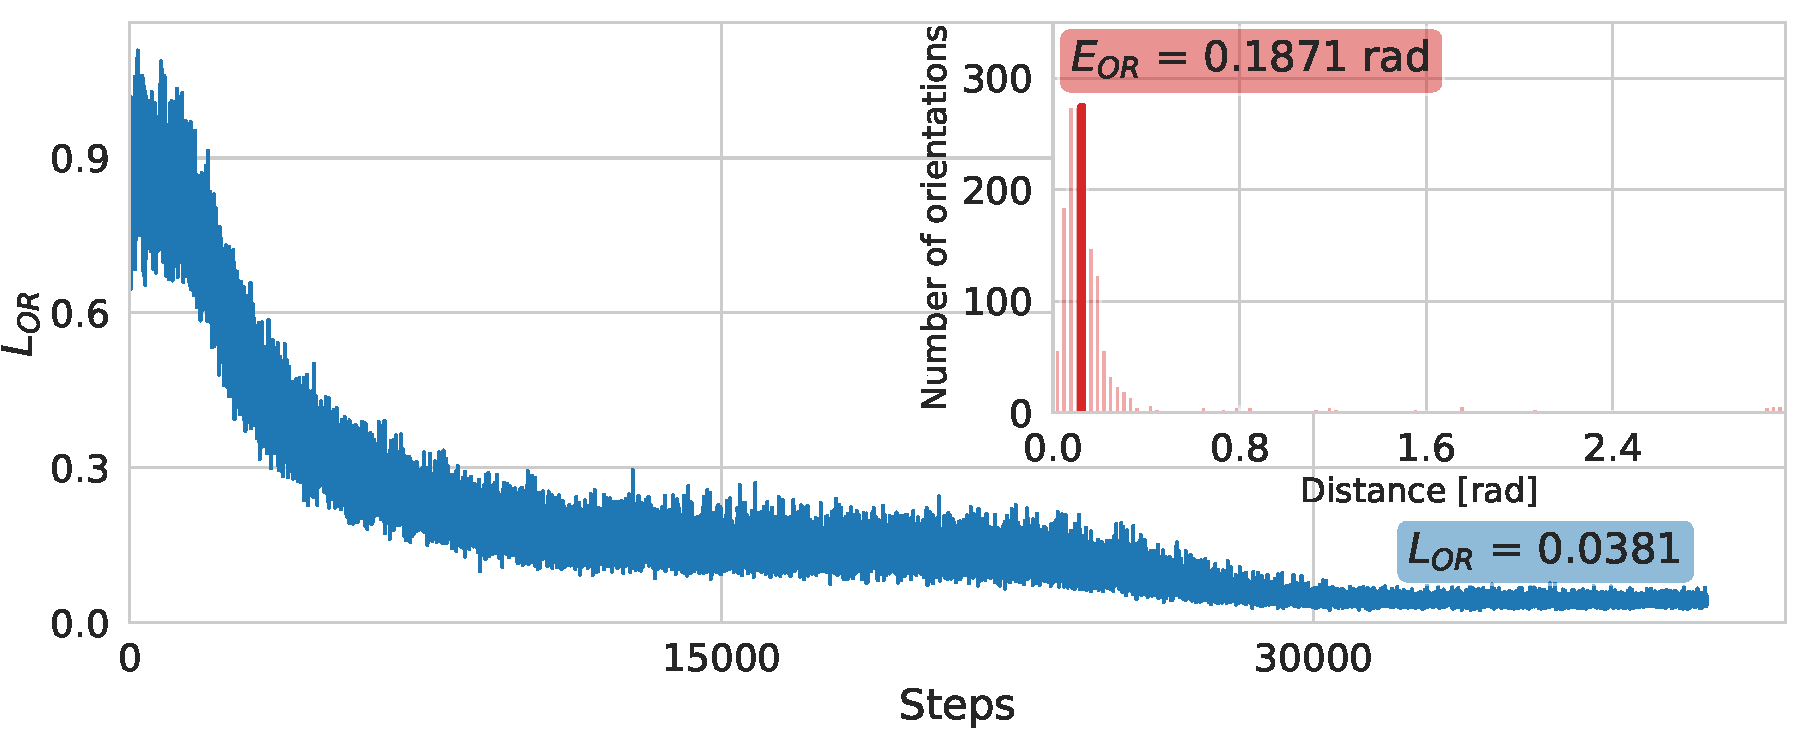
\includegraphics[height=8em]{figures/5a1a_noise0_ar_aa}
        \caption{Recovered $\{ \widehat{q_i} \}$ from $\{ \p_i = \mathbf{P}_{\bth_i} \x \}$, $\x$ from \texttt{5a1a}.}%
        \label{fig:5a1a-noise0-orientation-recovery}
    \end{subfigure}
    \hfill
    \begin{subfigure}[b]{0.26\linewidth}
        \centering
        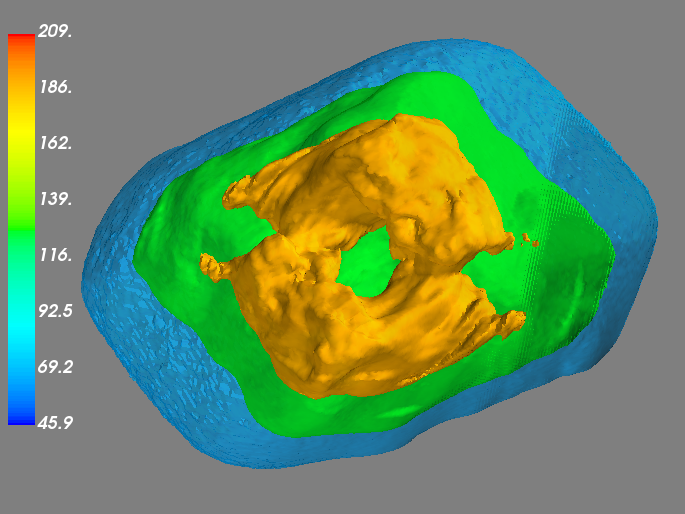
\includegraphics[height=8em]{figures/5a1a_aligned}
        \caption{Reconstructed $\widehat{\x}$ from $\{ \p_i, \widehat{q_i} \}$.}%
        \label{fig:5a1a-noise0-reconstruction-recovered}
    \end{subfigure}
    \hfill
    \begin{subfigure}[b]{0.26\linewidth}
        \centering
        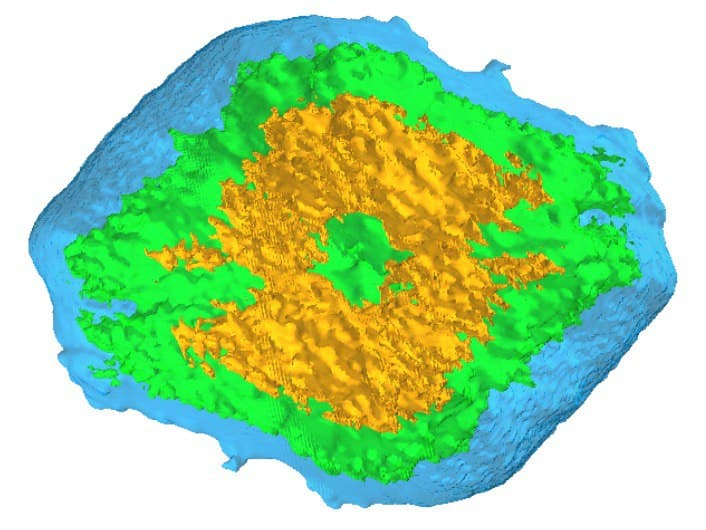
\includegraphics[height=8em]{figures/5a1a_ground_truth}
        \caption{Reconstructed $\widehat{\x}$ from $\{ \p_i, q_i \}$.}%
        \label{fig:5a1a-noise0-reconstruction-true}
    \end{subfigure}
    \caption{%
        Orientation recovery and density reconstruction from estimated distances.
        The first column~(a,d,g) shows orientation recovery:
        The blue curve shows the evolution of the recovery loss until convergence, with the minimum $L_\text{OR}$ \eqnref{orientation-recovery} highlighted.
        The red histogram shows the errors in the recovered orientations $\{d_q(q_i, \mathbf{T}\widehat{q_i})\}$, with the mean $E_\text{OR}$ \eqnref{orientation-recovery-error} highlighted.
    The second and third columns show density maps $\widehat{\x}$ reconstructed from projections $\{ \p_i \}$, and recovered orientations $\{ \widehat{q_i} \}$~(b,e,h) or true orientations $\{ q_i \}$~(c,f,i).
        % Explain columns then rows.
        The first row~(a,b,c) shows the process for noiseless projections $\p_i = \mathbf{P}_{\bth_i} \x$, where $\x$ comes from \texttt{5j0n}.
        \mdeff{Why is $L_\text{OR} = 0.05$ while it is $0.01$ in \figref{results:distance-estimation:noise}?\banjac{Thanks for notice! I didn't see that. I am rerunning this pipeline for this plot. Update: I reran the 5j0n pipeline with 0 and 16 noise variance and both are shifted by ~0.25 from the results we have in the noise tests... I am not sure why, however, my thinking is that it might be due to working with a different set of generated projections from the same protein (different train-val-test split). What do you think I should do? Should I write about it or rerun the noisy experiments }}
        The second row~(d,e,f) shows the process for noisy projections $\p_i = \mathbf{P}_{\bth_i} \x + \mathbf{n}$, where $\mathbf{n} \sim \mathcal{N}(0, \sigma^2\mathbf{I}), \sigma^2=16$, and $\x$ comes from \texttt{5j0n}.
        %\mdeff{$E_\text{OR}=0.4184$ is the same as for $\sigma^2=15$ (\figref{results:distance-estimation:noise}). Coincidence or error?}\banjac{Not coincidence. I  use the result from variance 16 for variance 15 on variance plot. I fill fix it to 16 in 9b}
        The third row~(g,h,i) shows the process for noiseless projections $\p_i = \mathbf{P}_{\bth_i} \x$, where $\x$ comes from \texttt{5a1a}.
        \mdeff{It would be clearer here to have $P_{q_i}$ instead of $P_{\bth_i}$ but we didn't introduce this notation. Should we?}\banjac{IMO: Since our goal is to provide the microscope with 3 euler angles, and since ASTRA is using euler angles to generate the projections, I would leave $\bth$. Laurene what do you think?}\lau{Actually I would just remove the use of the operator in the legend; it's not necessary, plus it allows us to avoid this confusion. In particular, I would not use $P_{\bth_i}$ in the captions, it clashes with the quaternion notation in a big way.}
    }
\end{figure}

\figref{5j0n-noise0-orientation-recovery} shows the recovery of orientations from distances estimated from clean projections of \texttt{5j0n}.
A mean error of $E_\text{OR} \approx 0.16$ radians ($\approx 9\degree$) in the recovered orientations led to a \todo{pretty good?} reconstruction (\figref{5j0n-noise0-reconstruction-recovered}) compared to that with true orientations (\figref{5j0n-noise0-reconstruction-true}).
\mdeff{I'm not sure how to qualify the reconstructed density maps.} \lau{I'm not sure we should try to be honest. The only thing we could do is give its resolution.}
\todo{Don't qualify in absolute terms, but say how adding noise results in a reconstruction of lower resolution.}

As expected from the experiments in \secref{results:distance-estimation:sensitivity}, adding white noise with variance $\sigma^2=16$ to the projections worsen the recovered orientations (\figref{5j0n-noise16-orientation-recovery}) to a mean error of $E_\text{OR} \approx 0.42$ radians ($\approx 24\degree$).
That leads to a \todo{worse/lower resolution/blurrier} reconstruction (\figref{5j0n-noise16-reconstruction-recovered}).
Note that reconstructing from true orientations worsen too  (\figref{5j0n-noise16-reconstruction-true}) as the projections themselves are degraded.

Finally, \figref{5a1a-noise0-orientation-recovery} shows the recovery of orientations from clean projections of \texttt{5a1a}.
A mean error of $E_\text{OR} \approx 0.19$ radians ($\approx 11\degree$) in the recovered orientations led to a \todo{blurrier} reconstruction (\figref{5j0n-noise0-reconstruction-recovered}) compared to that with true orientations (\figref{5j0n-noise0-reconstruction-true}).
Orientation recovery is slightly more difficult for this protein \todo{as distance estimation is more difficult because} \mdeff{Symmetries? Something else? What makes \texttt{5a1a} harder than \texttt{5j0n}?}.

%We observe that the recovery of more accurate orientations lead to the reconstruction of more accurate density maps.
%Hence, the estimation of more accurate distances lead to more accurate reconstructions.
We observe that the estimation of more accurate distances not only lead to the recovery of more accurate orientations, but also to the reconstruction of more accurate density maps.
%Reconstruction is most affected by the presence of noise, due to the degraded estimation of distances.
We are hence confident that reconstruction would substantially improve if a more powerful SiameseNN would be trained on more data for distance estimation (and a \todo{more serious/advanced/less naive?} \lau{more robust} method used for reconstruction).
%\mdeff{Story: pipeline works but better distance estimation is needed for SOTA reconstruction.
%Method is however promising because learned distance is robust to perturbations and recovery works if distance works.}
